\documentclass[twocolumn,twoside,10pt,a4paper]{article}

\usepackage[portuguese]{babel}  % portuguese
\usepackage{graphicx}           % images: .png or .pdf w/ pdflatex; .eps w/ latex

%% For iso-8859-1 (latin1), comment next line and uncomment the second line
\usepackage[utf8]{inputenc}
%\usepackage[latin1]{inputenc}

\usepackage[T1]{fontenc}        % T1 fonts
\usepackage{lmodern}            % fonts
%\usepackage{times}              % PS fonts
\usepackage{lastpage}           % to have lastpage in headers
\usepackage{url}                % urls

% geometry package
\usepackage[outer=20mm,inner=30mm,vmargin=20mm,includehead,includefoot,headheight=15pt]{geometry}

%% space between columns
\columnsep 10mm

% avoid widows and orphans
\clubpenalty=300
\widowpenalty=300

\usepackage[pdftex]{hyperref}
\hypersetup{%
    a4paper = true,              % use A4 paper 
    bookmarks = true,            % make bookmarks 
    colorlinks = true,           % false: boxed links; true: colored links
    pdffitwindow = false,        % page fit to window when opened
    pdfpagemode = UseNone,       % do not show bookmarks
    pdfpagelayout = SinglePage,  % displays a single page
    pdfpagetransition = Replace, % page transition
    linkcolor=blue,              % hyperlink colors
    urlcolor=blue,
    citecolor=blue,
    anchorcolor=green
}

\usepackage{indentfirst}       % indent also 1st paragraph

\pagestyle{myheadings}         % Option to put page headers
\markboth{{\small\it Exemplo de artigo em \LaTeX}}
{{\small\it Grupo xx, \today}}

%\hyphenation{}                  % explicit hyphenation

% entities
\newcommand{\class}[1]{{\normalfont\slshape #1\/}}
\newcommand{\svg}{\class{SVG}}
\newcommand{\scada}{\class{SCADA}}
\newcommand{\scadadms}{\class{SCADA/DMS}}

\title{JogginGo! }

\author{Luís Carlos Moreira Dias\\
\small Faculdade de Engenharia\\[-0.8ex]
\small da Universidade do Porto\\[-0.8ex]
\small R.\ Dr.\ Roberto Frias, 4200-465 Porto\\[-0.8ex]
\small \texttt{ei08094@fe.up.pt}\\
\and
Luís Filipe Castanheira Gomes\\
\small Faculdade de Engenharia\\[-0.8ex]
\small da Universidade do Porto\\[-0.8ex]
\small R.\ Dr.\ Roberto Frias, 4200-465 Porto\\[-0.8ex]
\small \texttt{ei08169@fe.up.pt}
}

\date{\today}

\begin{document}

\maketitle
\thispagestyle{plain} 

\begin{abstract}
Com uma interface limpa e amiga do utilizador, o JogginGo! é uma aplicação Web que permite a gestão de todas as corridas feitas por qualquer utilizador registado. Cada corrida, é um tratada como um conjunto de coordenadas GPS (\textit{Global Positioning System}) recolhidas com o auxílio de um dispositivo móvel. A cada minuto, é recolhida a posição em que o atleta se encontra, para uma mais fácil representação no \textit{webservice}. Para além disso será ainda possível competir contra outros utilizadores, através de contra-relógio, em percursos pré-definidos pela plataforma. 
\end{abstract}

\section{Introdução}\label{sec:intro}

Os sistemas \scada{} (\emph{Supervisory Control And Data Acquisition})
são responsáveis pela recolha e análise de informação em tempo real.
Actualmente estes sistemas recorrem às mais avançadas tecnologias de
computação e comunicação para monitorizar e controlar estruturas ou
equipamentos industriais dispersos geograficamente e recorrem a
interfaces gráficas para tornar a interacção com o utilizador mais
amigável\footnote{Exemplo de artigo retirado de uma submissão à
  Conferência XATA2006, mas sem usar LLNCS.}.

Lorem ipsum dolor sit amet, consectetuer adipiscing elit. Nunc eu
nulla. Pellentesque vitae nibh ultrices quam iaculis
convallis. Aliquam purus eros, varius eget, volutpat sodales,
imperdiet nec, lacus. Curabitur in elit sed sem rutrum posuere. Class
aptent taciti sociosqu ad litora torquent per conubia nostra, per
inceptos himenaeos. Duis sem. Praesent ultricies odio vel
sapien. Integer faucibus malesuada libero. Cras semper, dolor id
ullamcorper varius, magna risus volutpat felis, id pellentesque nulla
ante at erat. Integer sodales. 

Quisque sit amet odio. In at risus sit amet turpis interdum
posuere. Maecenas iaculis vehicula sem. Ut leo arcu, malesuada vel,
imperdiet id, dignissim a, purus. Duis eleifend, lectus non venenatis
dignissim, risus libero imperdiet mi, nec gravida massa libero sed
mauris. Nullam lobortis libero non sapien. Integer convallis iaculis
erat. Morbi dictum. Ut ultrices pellentesque velit. Cras ac
ante. Etiam in neque tincidunt lacus gravida vehicula. Proin et nisi. 

Vivamus non nunc nec risus tempor varius. Quisque bibendum mi at
dolor. Aliquam consectetuer condimentum risus. Aliquam luctus pulvinar
sem. Duis aliquam, urna et vulputate tristique, dui elit aliquet nibh,
vel dignissim magna turpis id sapien. Duis commodo sem id
quam. Phasellus dolor. Class aptent taciti sociosqu ad litora torquent
per conubia nostra, per inceptos himenaeos. 

Duis eget diam. In est justo, tristique in, lacinia vel, feugiat eget,
quam. Pellentesque habitant morbi tristique senectus et netus et
malesuada fames ac turpis egestas. Fusce feugiat, elit ac placerat
fermentum, augue nisl ultricies eros, id fringilla enim sapien eu
felis. Vestibulum ante ipsum primis in faucibus orci luctus et
ultrices posuere cubilia Curae; Sed dolor mi, porttitor quis,
condimentum sed luctus. 

Para além desta introdução, onde se caracterizou o problema abordado
por este projecto, refere-se na secção~\ref{sec:sota} o
estado da arte e são descritos os trabalhos relacionados com a
visualização de diagramas sinópticos de sistemas \scada{} na
\textit{Web}. 

\section{\svg}\label{sec:sota}

Nos últimos tempos têm surgido diversas soluções, apresentadas por
empresas do sector Automação de Sistemas para a disponibilização de
sistemas \scadadms{} na \textit{Web}.

\emph{Scalable Vector Graphics} é uma linguagem em formato XML que
descreve gráficos de duas dimensões. 
Este formato padronizado pela W3C (\emph{World Wide Web Consortium})
é livre de patentes ou direitos de autor e está totalmente
documentado, à semelhança de outros W3C standards~\cite{kn:svgdoc}.

Sendo uma linguagem XML, o \svg{} herda uma série de vantagens: a
possibilidade de transformar \svg{} usando técnicas como XSLT, de embeber
\svg{} em qualquer documento XML usando \textit{namespaces} ou até de 
estilizar \svg{} recorrendo a CSS (\emph{Cascade Style Sheets}). 
De uma forma geral, pode dizer-se que \svg{}s interagem bem com as
actuais tecnologias ligadas ao XML e à Web, tal como referido
em~\cite{kn:svgibm,kn:svgw3c}.

% Duis eget diam. In est justo, tristique in, lacinia vel, feugiat eget,
% quam. Pellentesque habitant morbi tristique senectus et netus et
% malesuada fames ac turpis egestas. Fusce feugiat, elit ac placerat
% fermentum, augue nisl ultricies eros, id fringilla enim sapien eu
% felis. Vestibulum ante ipsum primis in faucibus orci luctus et
% ultrices posuere cubilia Curae; Sed dolor mi, porttitor quis,
% condimentum sed luctus. 

\subsection{Batik \svg{} Toolkit} \label{batik} 

Batik é um conjunto de bibliotecas baseadas em \textit{Java} que
permitem o uso de imagens \svg{} (visualização, geração ou
manipulação) em aplicações ou \textit{applets} \cite{kn:batikarchitecture}.  
O projecto Batik destina-se a fornecer ao programador alguns módulos
que permitem desenvolver soluções especificas usando \svg. 

Loren ipsum dolor sit amet, consectetuer adipiscing elit. 
Praesent sit amet sem. Maecenas eleifend facilisis leo. Vestibulum et
mi. Aliquam posuere, ante non tristique consectetuer, dui elit
scelerisque augue, eu vehicula nibh nisi ac est. Suspendisse elementum
sodales felis. Nullam laoreet fermentum urna. 

Duis eget diam. In est justo, tristique in, lacinia vel, feugiat eget,
quam. Pellentesque habitant morbi tristique senectus et netus et
malesuada fames ac turpis egestas. Fusce feugiat, elit ac placerat
fermentum, augue nisl ultricies eros, id fringilla enim sapien eu
felis. Vestibulum ante ipsum primis in faucibus orci luctus et
ultrices posuere cubilia Curae; Sed dolor mi, porttitor quis,
condimentum sed luctus. 

\section{Visualizador de Sinópticos}\label{sec:application}

A arquitectura do visualizador assenta sobre os seguintes conceitos base \cite{kn:zpmd}:
\begin{itemize}
\item \textbf{Componentes} --- Suspendisse auctor mattis augue \emph{push};
\item \textbf{Praesent} --- Sit amet sem maecenas eleifend facilisis leo;
\item \textbf{Pellentesque} --- Habitant morbi tristique senectus et netus.
\end{itemize}

Duis eget diam. In est justo, tristique in, lacinia vel, feugiat eget,
quam. Pellentesque habitant morbi tristique senectus et netus et
malesuada fames ac turpis egestas. Fusce feugiat, elit ac placerat
fermentum, augue nisl ultricies eros, id fringilla enim sapien eu
felis. Vestibulum ante ipsum primis in faucibus orci luctus et
ultrices posuere cubilia Curae; Sed dolor mi, porttitor quis,
condimentum sed luctus. 

Apresenta-se de seguida um exemplo de equação, completamente fora do contexto:
\begin{eqnarray}
CIF_1: \hspace*{5mm}F_0^j(a) &=& \frac{1}{2\pi \iota} \oint_{\gamma} \frac{F_0^j(z)}{z - a} dz\\
CIF_2: \hspace*{5mm}F_1^j(a) &=& \frac{1}{2\pi \iota} \oint_{\gamma} \frac{F_0^j(x)}{x - a} dx \label{eq:cif}
\end{eqnarray}

Na Equação~\ref{eq:cif} lorem ipsum dolor sit amet, consectetuer
adipiscing elit. Suspendisse tincidunt viverra elit. Donec tempus
vulputate mauris. Donec arcu. Vestibulum condimentum porta
justo. Curabitur ornare tincidunt lacus. Curabitur ac massa vel ante
tincidunt placerat. Cras vehicula semper elit. Curabitur gravida, est
a elementum suscipit, est eros ullamcorper quam, sed cursus velit
velit tempor neque. Duis tempor condimentum ante.

\subsection{Exemplo de Figura}

É apresentado na Figura~\ref{fig:arch} %da página~\pageref{fig:arch}
um exemplo de figura flutuante que ficará onde o \LaTeX\ entender.

\begin{figure}
  \begin{center}
    \leavevmode
    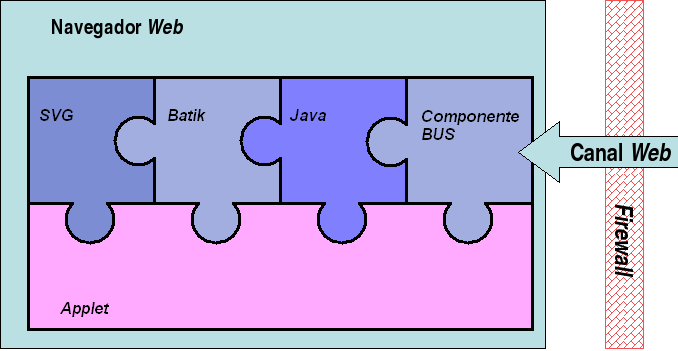
\includegraphics[width=0.45\textwidth]{puzzle}
    \caption{Arquitectura da Solução Proposta}
    \label{fig:arch}
  \end{center}
\end{figure}

Loren ipsum dolor sit amet, consectetuer adipiscing elit. 
Praesent sit amet sem. Maecenas eleifend facilisis leo. Vestibulum et
mi. Aliquam posuere, ante non tristique consectetuer, dui elit
scelerisque augue, eu vehicula nibh nisi ac est. Suspendisse elementum
sodales felis. Nullam laoreet fermentum urna. 

Duis eget diam. In est justo, tristique in, lacinia vel, feugiat eget,
quam. Pellentesque habitant morbi tristique senectus et netus et
malesuada fames ac turpis egestas. Fusce feugiat, elit ac placerat
fermentum, augue nisl ultricies eros, id fringilla enim sapien eu
felis. Vestibulum ante ipsum primis in faucibus orci luctus et
ultrices posuere cubilia Curae; Sed dolor mi, porttitor quis,
condimentum sed luctus. 

Duis eget diam. In est justo, tristique in, lacinia vel, feugiat eget,
quam. Pellentesque habitant morbi tristique senectus et netus et
malesuada fames ac turpis egestas. Fusce feugiat, elit ac placerat
fermentum, augue nisl ultricies eros, id fringilla enim sapien eu
felis. Vestibulum ante ipsum primis in faucibus orci luctus et
ultrices posuere cubilia Curae; Sed dolor mi, porttitor quis,
condimentum sed luctus. 

\subsection{Exemplo de Tabela}

É apresentado na Tabela~\ref{tab:exemplo1} um exemplo de tabela.

\begin{table}[h]
  \centering
  \caption{Uma Tabela Simples}
\begin{tabular}{| l | p{45mm} |}
	\hline
\textbf{Acrónimo} & \textbf{Significado}\\
	\hline
	\hline
        ADT   & \emph{Abstract Data Type}\\\hline
        ANDF  & \emph{Architecture-Neutral Distribution Format}\\\hline
        API   & \emph{Application Programming Interface}\\
	\hline
\end{tabular}
  \label{tab:exemplo1}
\end{table}

Duis eget diam. In est justo, tristique in, lacinia vel, feugiat eget,
quam. Pellentesque habitant morbi tristique senectus et netus et
malesuada fames ac turpis egestas. Fusce feugiat, elit ac placerat
fermentum, augue nisl ultricies eros, id fringilla enim sapien eu
felis. Vestibulum ante ipsum primis in faucibus orci luctus et
ultrices posuere cubilia Curae; Sed dolor mi, porttitor quis,
condimentum sed luctus. 

Loren ipsum dolor sit amet, consectetuer adipiscing elit. 
Praesent sit amet sem. Maecenas eleifend facilisis leo. Vestibulum et
mi. Aliquam posuere, ante non tristique consectetuer, dui elit
scelerisque augue, eu vehicula nibh nisi ac est. Suspendisse elementum
sodales felis. Nullam laoreet fermentum urna. 

Duis eget diam. In est justo, tristique in, lacinia vel, feugiat eget,
quam. Pellentesque habitant morbi tristique senectus et netus et
malesuada fames ac turpis egestas. Fusce feugiat, elit ac placerat
fermentum, augue nisl ultricies eros, id fringilla enim sapien eu
felis. Vestibulum ante ipsum primis in faucibus orci luctus et
ultrices posuere cubilia Curae; Sed dolor mi, porttitor quis,
condimentum sed luctus. 

% \begin{table}
%   \centering
%   \caption{Tabela Exemplo}
% \begin{tabular}{|c|r@{.}lr@{.}lr@{.}l||r|}
% 	\hline
% \multicolumn{8}{|c|}
% 	{\rule[-3mm]{0mm}{8mm}Iteração $k$ de $f(x_n)$} \\
% \textbf{\em k}
% 	& \multicolumn{2}{c}{$x_1^k$}
% 	& \multicolumn{2}{c}{$x_2^k$}
% 	& \multicolumn{2}{c||}{$x_3^k$}
% 	& comentários \\ \hline \hline
% 0   & -0&3                 & 0&6                 &  0&7   & - \\
% 1   &  0&47102965 & 0&04883157 & -0&53345964  & $\delta<\epsilon$ \\
% 2   &  0&49988691 & 0&00228830 & -0&52246185  & $\delta < \varepsilon$ \\
% 3   &  0&49999976 & 0&00005380 & -0&523656   &   $N$ \\
% 4   &  0&5                 & 0&00000307 & -0&52359743  & \\
% \vdots	& \multicolumn{2}{c}{\vdots}
% 	& \multicolumn{2}{c}{$\ddots$}
% 	& \multicolumn{2}{c||}{\vdots}  & \\
% 7   &  0&5   & 0&0    & \textbf{-0}&\textbf{52359878}
% 		 & $\delta<10^{-8}$ \\ \hline
% \end{tabular}
%   \label{tab:exemplo2}
% \end{table}

% Loren ipsum dolor sit amet, consectetuer adipiscing elit. 
% Praesent sit amet sem. Maecenas eleifend facilisis leo. Vestibulum et
% mi. Aliquam posuere, ante non tristique consectetuer, dui elit
% scelerisque augue, eu vehicula nibh nisi ac est. Suspendisse elementum
% sodales felis. Nullam laoreet fermentum urna. 

Duis eget diam. In est justo, tristique in, lacinia vel, feugiat eget,
quam. Pellentesque habitant morbi tristique senectus et netus et
malesuada fames ac turpis egestas. Fusce feugiat, elit ac placerat
fermentum, augue nisl ultricies eros, id fringilla enim sapien eu
felis. Vestibulum ante ipsum primis in faucibus orci luctus et
ultrices posuere cubilia Curae; Sed dolor mi, porttitor quis,
condimentum sed luctus. 

\section{Conclusões}\label{sec:conclusions}

Neste artigo abordou-se o desenvolvimento de um protótipo, com vista a
estudar a adequadibilidade da tecnologia \svg{} à visualização de
sinópticos na \textit{Web}.

Loren ipsum dolor sit amet, consectetuer adipiscing elit. 
Praesent sit amet sem. Maecenas eleifend facilisis leo. Vestibulum et
mi. Aliquam posuere, ante non tristique consectetuer, dui elit
scelerisque augue, eu vehicula nibh nisi ac est. Suspendisse elementum
sodales felis. Nullam laoreet fermentum urna. 

Duis eget diam. In est justo, tristique in, lacinia vel, feugiat eget,
quam. Pellentesque habitant morbi tristique senectus et netus et
malesuada fames ac turpis egestas. Fusce feugiat, elit ac placerat
fermentum, augue nisl ultricies eros, id fringilla enim sapien eu
felis. Vestibulum ante ipsum primis in faucibus orci luctus et
ultrices posuere cubilia Curae; Sed dolor mi, porttitor quis,
condimentum sed luctus. 

%% auto bibliographic list 
\renewcommand{\bibname}{Referências}
% uses bibtex file
%\bibliographystyle{alpha-pt}
%\bibliographystyle{alpha}
\bibliographystyle{unsrt-pt}
%\bibliographystyle{unsrt}
\bibliography{artigo}

\end{document}


